\documentclass[11pt]{article}
\usepackage{UF_FRED_paper_style}
\usepackage{apacite}
\usepackage{makecell}%To keep spacing of text in tables
\setcellgapes{4pt}%parameter for the spacing
\usepackage{lipsum} %% Package to create dummy text (comment or erase before start)

\usepackage{hyperref}
\hypersetup{
    colorlinks=true,
    linkcolor=blue,
    filecolor=magenta,
    urlcolor=cyan,
}

%% ===============================================
%% Setting the line spacing (3 options: only pick one)
% \doublespacing
% \singlespacing
\onehalfspacing
%% ===============================================

\setlength{\droptitle}{-5em} %% Don't touch

% %%%%%%%%%%%%%%%%%%%%%%%%%%%%%%%%%%%%%%%%%%%%%%%%%%%%%%%%%%
% SET THE TITLE
% %%%%%%%%%%%%%%%%%%%%%%%%%%%%%%%%%%%%%%%%%%%%%%%%%%%%%%%%%%

% TITLE:
\title{Fake or Not: Detecting Manipulated Images with Deep Learning}

% AUTHORS:
\author{Alena Kalodzitsa\\% Name author
    \href{mailto:alena.kalodzitsa@duke.edu}{\texttt{alena.kalodzitsa@duke.edu}} %% Email author 1
\and Amandeep Rathee\\% Name author
    \href{mailto:amandeep.rathee@duke.edu}{\texttt{amandeep.rathee@duke.edu}} %% Email author 2
\and Juan David Martinez\\% Name author
    \href{mailto:jdavid.martinez@duke.edu}{\texttt{jdavid.martinez@duke.edu}}%% Email author 3
\and  Shota Takeshima\\% Name author
    \href{mailto:shota.takeshima@duke.edu}{\texttt{shota.takeshima@duke.edu}}%%
\and  Xiao Lu\\% Name author
    \href{mailto:xiao.lu@duke.edu}{\texttt{xiao.lu@duke.edu}}%%
    }

% DATE:
\date{\today}

\urlstyle{same}

\clubpenalty = 10000
\widowpenalty = 50000
\displaywidowpenalty = 50000

% %%%%%%%%%%%%%%%%%%%%%%%%%%%%%%%%%%%%%%%%%%%%%%%%%%%%%%%%%%
% %%%%%%%%%%%%%%%%%%%%%%%%%%%%%%%%%%%%%%%%%%%%%%%%%%%%%%%%%%
\begin{document}
% %%%%%%%%%%%%%%%%%%%%%%%%%%%%%%%%%%%%%%%%%%%%%%%%%%%%%%%%%%
% %%%%%%%%%%%%%%%%%%%%%%%%%%%%%%%%%%%%%%%%%%%%%%%%%%%%%%%%%%
% ABSTRACT
% %%%%%%%%%%%%%%%%%%%%%%%%%%%%%%%%%%%%%%%%%%%%%%%%%%%%%%%%%%
% %%%%%%%%%%%%%%%%%%%%%%%%%%%%%%%%%%%%%%%%%%%%%%%%%%%%%%%%%%
{\setstretch{.8}
\maketitle
% %%%%%%%%%%%%%%%%%%
\begin{abstract}
% CONTENT OF ABS HERE--------------------------------------

Digital images are essential to how humankind uses the internet, from saving and sharing memories to reporting news and serve as the cornerstone of e-commerce. Entire websites, based solely on image sharing, experience daily uploads of pictures surpassing the tenths of millions. However, this ubiquitous access to digital imagery online has enabled the upsurge of image tampering, helping societal issues, such as identity theft or fake news, to thrive more effectively. The public's trust in digital photography has, therefore, compelling reasons to have plummeted. We aim for a fast and reliable approach to detect whether an image has been manipulated. Our method starts with 22 thousand images from the famous subreddit {\it PhotoshopBattles}, which later are transformed with Error Level Analysis and used to train a Convolutional Neural Network. As a result, this pipeline achieves better and faster results compared to human performance, offering an improved way to detect image manipulation at scale.

% END CONTENT ABS------------------------------------------
\end{abstract}
}

% %%%%%%%%%%%%%%%%%%%%%%%%%%%%%%%%%%%%%%%%%%%%%%%%%%%%%%%%%%
% %%%%%%%%%%%%%%%%%%%%%%%%%%%%%%%%%%%%%%%%%%%%%%%%%%%%%%%%%%
% BODY OF THE DOCUMENT
% %%%%%%%%%%%%%%%%%%%%%%%%%%%%%%%%%%%%%%%%%%%%%%%%%%%%%%%%%%
% %%%%%%%%%%%%%%%%%%%%%%%%%%%%%%%%%%%%%%%%%%%%%%%%%%%%%%%%%%

% --------------------
\section{Introduction}
% --------------------

Back in 1957 when Russell Kirsch produced the first digital image portraying his son, it was beyond imagination the impact this novel technology would have on humankind (Kirsch et al., 1957). Not long after, in 1982, the emergence of the Internet as we know it, became a reality thanks to the standardization of interconnected networks protocols (Frazer, 1996) and kickstarted a new paradigm in modern society. However, the popularization of digital photography only started when the JPEG file format was introduced in 1992, allowing digital images to be efficiently compressed making its usage more practical through the world wide web (Standard, 1992). These three important milestones defined how we engage, communicate and consume online nowadays. Digital imagery constitutes most of the web’s frontend, whenever we wish to buy a product online, hear a song, read a news article or even plan a vacation an image is crucial for a compelling user experience. Just In 2014, people uploaded an average of 1.8 billion digital images every single day adding up to 657 billion photos per year (Eveleth, 2015).

However, the proliferation of digital pictures has enabled and inspired the creation of image editing software such as Adobe Photoshop, Rebelle, Pixelmator, among others. Thanks to this,  digital retouching has become as pervasive as digital images. The danger comes when this retouching is used unethically to deceive or persuade viewers of non-real events. The above fuels the spread of societal issues such as fake news and identity theft.

Some manipulated images are easy to spot given their rustic or amateur editing process. Nonetheless, professional manipulations become harder to detect and require longer observation. In fact, it has been shown that humans are indeed quite inaccurate when detecting tampered images. On average, humans can effectively detect 65\% of fake images and take approximately one minute to judge (Nightingale et al., 2017). For these reasons, the credibility of an online image and its derived information is usually very low amongst viewers (Shen et al., 2019).

There is a clear need for a faster and more accurate way to detect manipulated images online and our study seeks to fulfill this need using a supervised learning approach to automatically classify an image as manipulated or not manipulated.


% --------------------
\section{Background}
% --------------------

There is a considerable body of literature on the subject of forgery detection and localization. With recent advancements in the computer vision field and acceleration of computing power, deep learning techniques became the primary tool to address forgery detection problems (Cozzolino et al., 2017). The literature review shows that several studies were conducted focusing on detecting one or only several particular manipulations in the image (Cozzolino et al., 2017). However, recently a more relevant line of research became to study detection methods that could detect all types of image manipulations. To illustrate, Gunawan et al. (2017) successfully implemented Error Level Analysis (ELA) to identify the location and the type of manipulation in the tampered images. They further enhanced ELA using vertical and horizontal histograms.  Whereas, Jeronymo et al. (2017) also demonstrated the effectiveness of the ELA method for forgery detection task, where the noisy components were removed from using the wavelet thresholding technique.

ELA produces a noise map, where images with greater noise indicate the forged regions. Despite the good performance of ELA, it has several limitations: (1) difficulty to process grayscale images, (2) high-frequency regions (e.g. hair and borders) can generate a lot of noise, which can be mistakenly interpreted as manipulated region, and (3) the method can only be applied to images with lossy compression (e.g. JPEG) (Jeronymo et al., 2017). Lastly, Sudiatmik et al. (2019) proposed a combination of ELA and VGG16 to detect a forged image, achieving 89\% accuracy on the validation set using the CASIA dataset.

To our knowledge, no previous research is done on image forgery detections methods trained on the PS-Battle dataset. It’s important to note that even though this dataset was not used to train the image forgery detection method, it was used in two recent studies for evaluating the performance of their pretrained models. A study by Wu et al. (2019) used the PS-Battle dataset to evaluate the generalizability of the ManTra-Net model, showing that it was successful at locating complex real-life forgeries. For the evaluation metric it used the image-level AUC, where the average likelihood of all pixels would indicate whether an image is manipulated. Depending on different settings, AUC ranged from 62\% to 76\%.

Another study by the European Commission (2019) applied the pretrained BusterNet, EXIL, QuadMani, and ManTra-Net models to the PS-Battles dataset, demonstrating decent results. However, this study primarily focused on localizing manipulated areas in the image rather than classifying whether an image is fake or not. Therefore, it would be challenging to compare the results of that study to ours.


% --------------------
\section{Data}
% --------------------

{\it PhotoshopBattles} is one of the most popular subreddits dedicated to photography on Reddit, with close to 13 million members. Digital photography aficionados gather around this thread to challenge themselves with all sorts of images. The dynamic is rather simple: someone posts an original picture and the community takes care of manipulating this picture to create creative derivative works. Our dataset has been previously collected from this thread using web scraping methods (Heller, 2018).

There are 11,142 original images and 90,886 modified versions of them. The latter means that each original image may have in most cases more than one photoshopped version. On average, there are eight photoshops for every original image. Given that the images are community-generated, their resolution, aspect ratio and color channels are not standardized.

Given that we make use of supervised learning to create our fake image detection algorithm, we used two labels (1: Manipulated/Fake, 0: Not Manipulated/Original) to tag each of the images available. We assume that the original picture has always the label Not Manipulated and all its derivative images are labeled as Manipulated based on the dynamics of the subreddit. However, in many cases, it is evident that even the original image has been manipulated before, which poses additional challenges to our study. Furthermore, the quality and variety of the retouches and manipulations is astonishingly high for many of the samples, adding level of complexity to our objective of training a fake image classifier with this data. Examples of original images and community-created derivatives are depicted in Figure 1.

Under the above labeling framework, our initial dataset of 102,028 images (in JPEG format) is significantly unbalanced, this would hurt the training process as our algorithm would be biased towards the {\it Manipulated} label. Only 10.9\% of samples correspond to the label 0 (Not manipulated/Original). To overcome this, we downsample the database of images and randomly select 11,142 manipulated images out of the total 90 thousand. As a result, our final dataset contains a total of 22,284 samples,  with perfectly balanced proportions of fake and original images.

\begin{figure}[!htb]
    \centering
        \includegraphics[scale=.55]{figures/figure_1.png}
    \caption{Example Images -- {\it PhotoshopBattles} dataset}
    \label{fig:1}
\end{figure}

% --------------------
\section{Methods}
% --------------------

At a high level, we used two techniques to tackle the problem of forgery detection: training CNNs from scratch, and using pre-trained networks, also known as transfer learning. While using each technique, we experimented with several CNN architectures. We also used several image preprocessing techniques to tackle the problem of forgery detection. Figure 2 shows a flowchart of the methodology that we followed.

\begin{figure}[!htb]
    \centering
        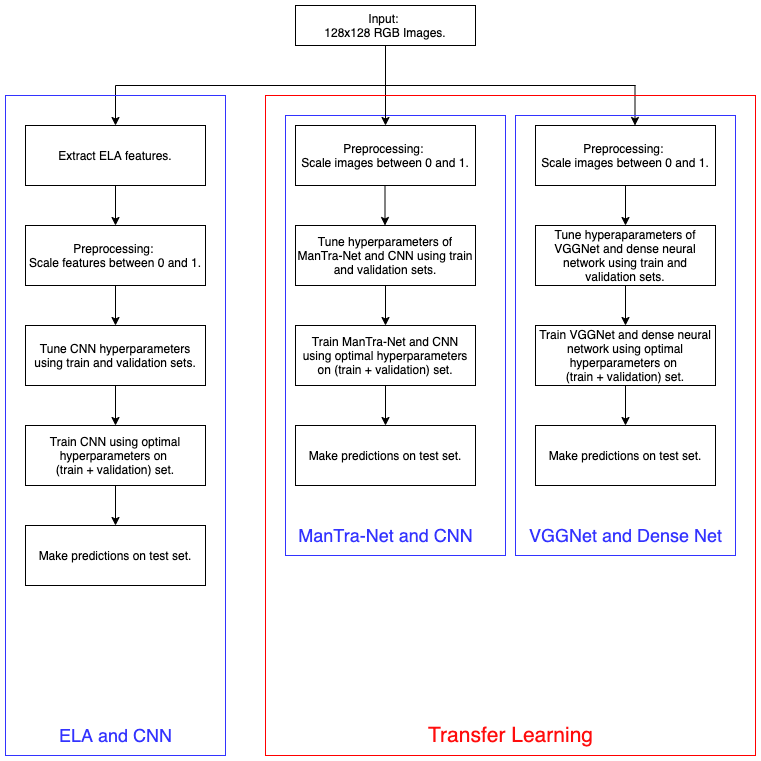
\includegraphics[scale=.55]{figures/figure_2.png}
    \caption{Flowchart of the methodology used in the report. The train, validation and test sets were consistent across all models.
}
    \label{fig:2}
\end{figure}

All 22,284 images were pre-processed by scaling each image into 128 x 128 to make the data more manageable and be able to iterate quickly over different methods with the computational resources at hand. Additionally, this dataset was divided into training data, validation data, and test dataset with a ratio of 70:15:15, making sure that the pair of images (original and fake) stay together in each dataset without shuffling.

%The exact number of images in each part might differ slightly since different image pre-processing techniques will have some images transformed unsuccessfully.

\subsection{Error level analysis and convolutional neural network}

We used a two-step strategy to classify forgery detection. First, we pre-processed images using ELA,  a forensic technique to identify digitally manipulated images. Then, we used the output of ELA to train multiple deep neural networks.

\subsubsection{Error level analysis}

ELA is a method for identifying the manipulated regions in the images. This method only can be applied to images with lossy compression such as images with JPEG format. When the image is saved in JPEG format, it has the same (or very similar) error level. When the image is resaved, however, the quality of image degrades at the same rate, introducing a similar error amount for the entire image. The quality of the image would degrade at each resaving. Therefore, the manipulated image would have altered the area at a higher error level compared to the remaining area of an image. Thus, after resaving an image with a particular quality, we can compare it to the original image and compute the difference in the level of compression, called error level.

This method is appropriate for our study because the fake images are digitally modified from its original version. In Figure 3, the modified areas (the gamified battlefield and audience) are indicated by brighter regions in its corresponding ELA version.

\begin{figure}[!htb]
    \centering
        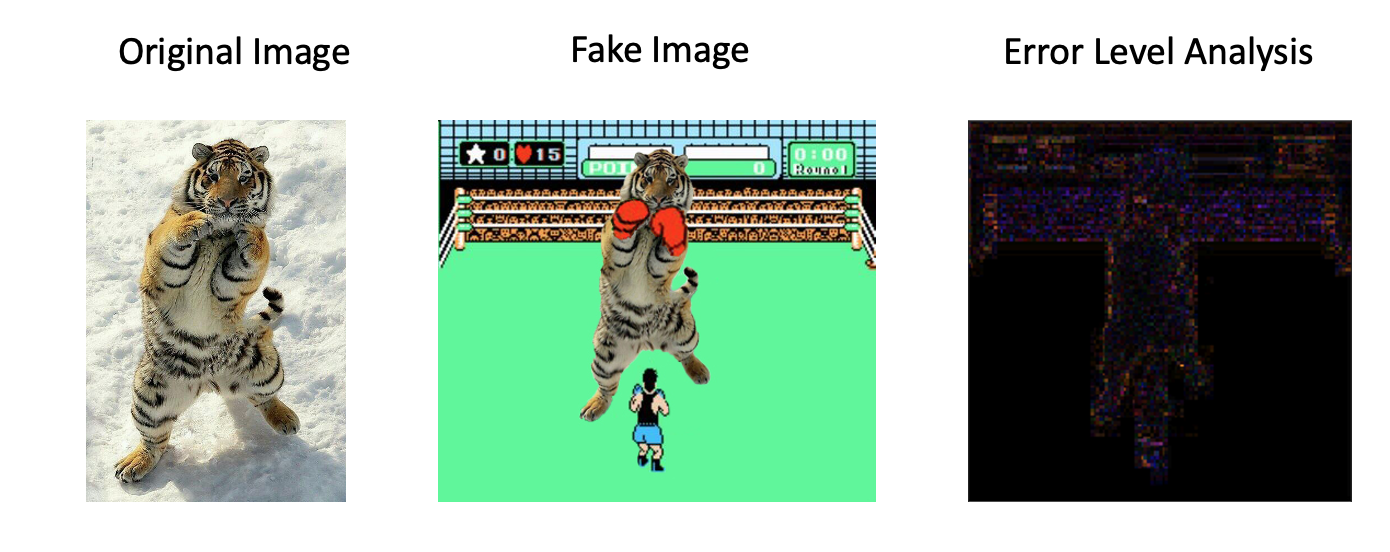
\includegraphics[scale=.62]{figures/figure_3.png}
    \caption{Examples of the original image and its ELA version.}
    \label{fig:3}
\end{figure}

ELA has one major hyperparameter: quality, a number between 0 and 100 to denote the quality in which the ELA image will be resaved. For ELA, the resaved image should have reduced quality,  and we chose the quality of 90 (producing the optimal results). When converting the images to ELA-transformed images, 50 images yielded errors and were dropped from the analysis. We also tried to tune this hyperparameter with some higher values for quality like 95 because we observed that a higher quality parameter will generate images with higher brightness and the highlighted areas are hence more obvious. We anticipated that these brighter ELA images will have better performance, which, however, achieved lower accuracy than a 90 quality ELA transformation. Thus, we continued the analysis using ELA with 90 for the quality parameter.

\subsubsection{Convolutional Neural Network}

Artificial neural networks (ANNs) have proven to be successful in automating various types of tasks. Convolutional neural networks (CNNs) are a type of ANNs that are extensively used in computer vision. Unlike a vanilla ANN, a CNN preserves the spatial structure of an image and looks at the image the way humans look at it. As a result, CNNs have achieved state-of-the-art results in many computer vision-related tasks today.

To classify original and fake images, we used a CNN with one input layer, three convolutional layers, one dense layer, and one output layer. We also added two max-pooling layers, two dropout layers and one flatten layer to our CNN. In Figure 4, we created a complete architecture of our model (using alexlenail.me software).

\begin{figure}[!htb]
    \centering
        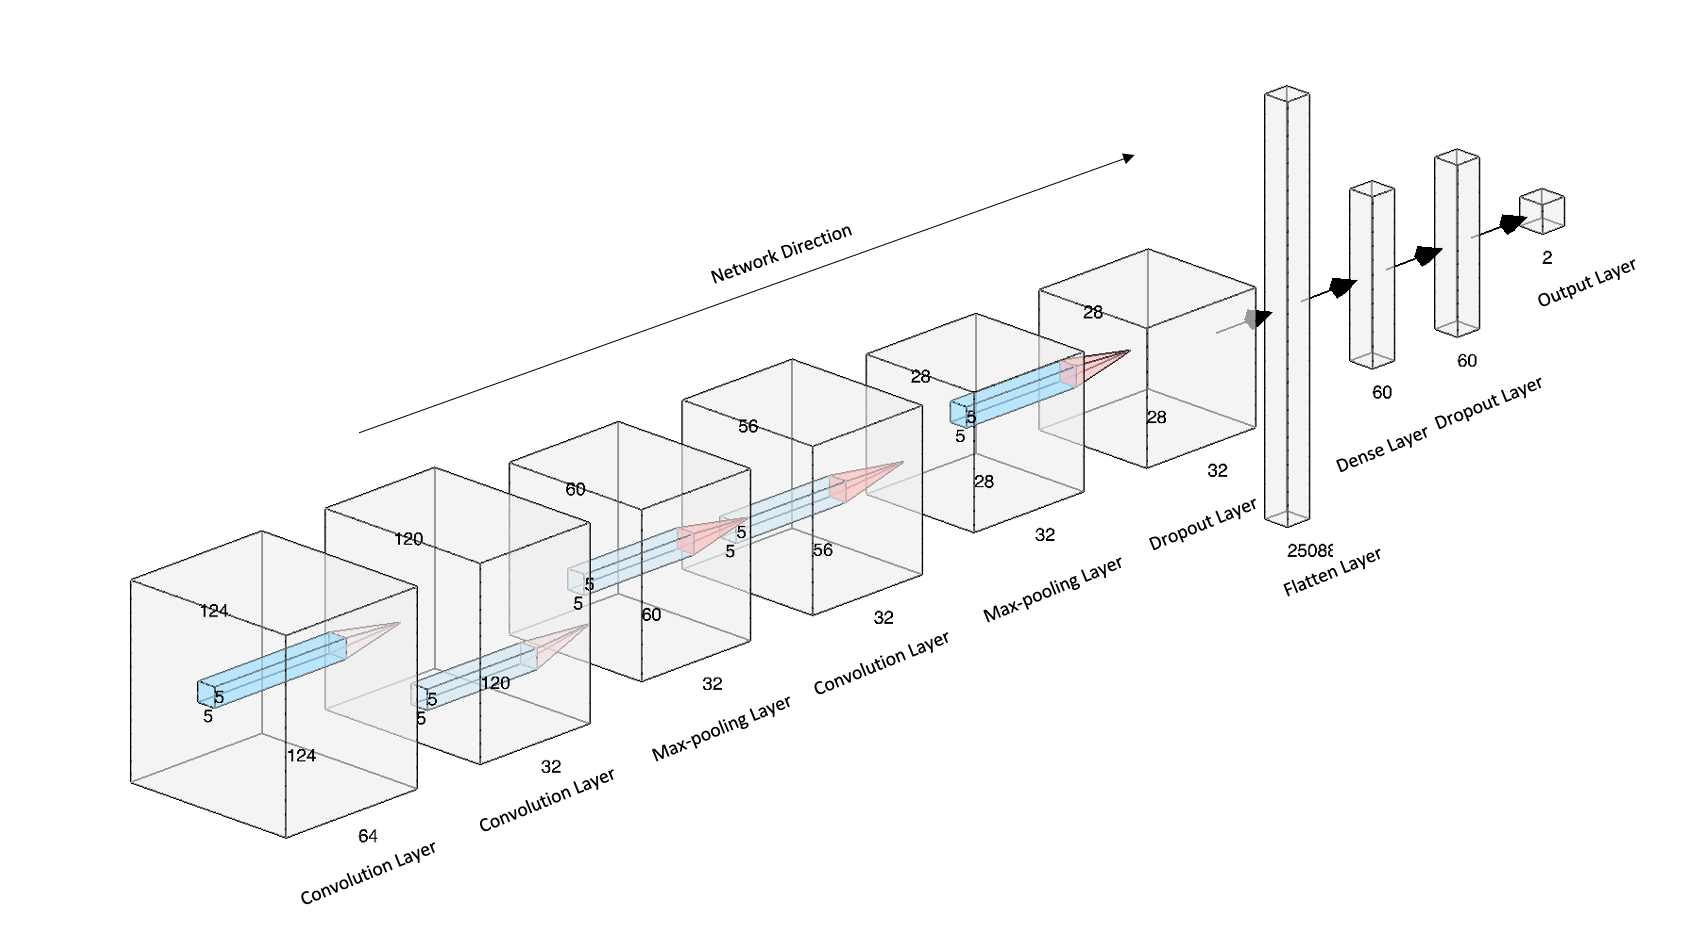
\includegraphics[scale=.50]{figures/figure_4.png}
    \caption{Complete architecture of the CNN used on top of ELA features.}
    \label{fig:4}
\end{figure}

Each convolutional operation is followed by a ReLu activation because this activation has proved to be effective in handling the gradient descent with less computation cost, helping the cost function converge quickly. And since we want a binary classification, in the end, we used sigmoid as the activation function for the output layer and set the cost function as binary cross-entropy.

A CNN has many hyperparameter choices such as the number of layers, number of filters in each layer. After a few trials, we chose to use 64 filters with a kernel size of 5x5 for the first convolution layer and 32 filters with a kernel size of 5x5 for the other two convolution layers. We also experimented with other filter sizes but 5x5 seems to work best in this classification task by giving the highest validation accuracy. Besides, to avoid overfitting to the training data, we also add L2 regularization with a lambda of 0.01 to the dense layer and the output layer. We used a batch size of 100, an epoch of 50 and a learning rate of 0.0005. These hyperparameters helped the model converge quickly, leading to the optimal performance as shown in the results section.

As presented in the flowchart shown in Figure 2, we tried several transfer learning methods besides the ELA and CNN pipeline to identify fake images. These methods include a ManTra-Net and CNN model, a VGGNet and dense net model, and a ResNet and dense net model. The broad pipeline for all these models is the same: choose a pre-trained model, train it on the training data and validate the performance on the validation set. Based on this performance, optimize the hyperparameters including (but not limited to) the choice of the model at the output layer of the pre-trained model, the number of layers, the number of neurons in each layer, activation functions, regularization techniques, and which layers in the pre-trained model should have their weights trainable. After finalizing the architecture and hyperparameters, we trained the models on all of the training and validation data and make predictions on test data. To see the detailed structure and methodology of these models, please refer to section 8.1 in the Appendix.

% --------------------
\section{Results}
% --------------------

We divided the dataset with 22,284 images into train, validation and test sets in the ratio of 70:15:15. Train and validation sets were used to find optimal architectures and hyperparameters for all models. We decided to use the following two metrics to measure the performance of all models: accuracy and area under the receiver operating characteristic (ROC) curve, also known as AUC. We used the accuracy metric to choose optimal models and their hyperparameters (while training and validating), and we report model performances on the test set in this section. We also realize that both the true positive rates and the false-positive rates are crucial for our classifiers, which is why we are using AUC of a ROC to report the model performances on the test set in this section. Further, AUC is a popular metric in deep learning and computer vision literature which allows comparison with previously used methods easier.

Table 1 shows the result of the three deep neural networks that we experimented with, as well as the human baselines (See Appendix). Figure 5 (left) shows the ROC curve for all three models. A precision-recall curve is also presented in Figure 5 (right) since it presents precision which is a useful metric to look at in a binary classification setting and makes comparisons easier. We choose not to report any metrics for the ResNet model and dense net model that we experimented with because its AUC and accuracy are both 0.5 on all three sets, and both these results are no better than chance.

\begin{table}[!htb]
    \centering
    \begin{tabular}{|l|l|l|}
    \hline
        \textbf{Model} & \textbf{Accuracy} & \textbf{AUC}\\ \hline
        Human aggregate model (baseline) & 73.8 $\pm$ 8.16 (95\% CI) & N/A \\ \hline
        Human ensemble & 82.0\% & N/A \\ \hline
        ELA and CNN & 71.2\% & 0.758 \\ \hline
        VGG16 and dense net & 51.8\% & 0.531 \\ \hline
        ManTra-Net and CNN & 57.7\% & 0.599 \\ \hline
    \end{tabular}
\caption{Accuracy and AUC of methods used.}
\end{table}

\begin{figure}[!htb]
    \centering
        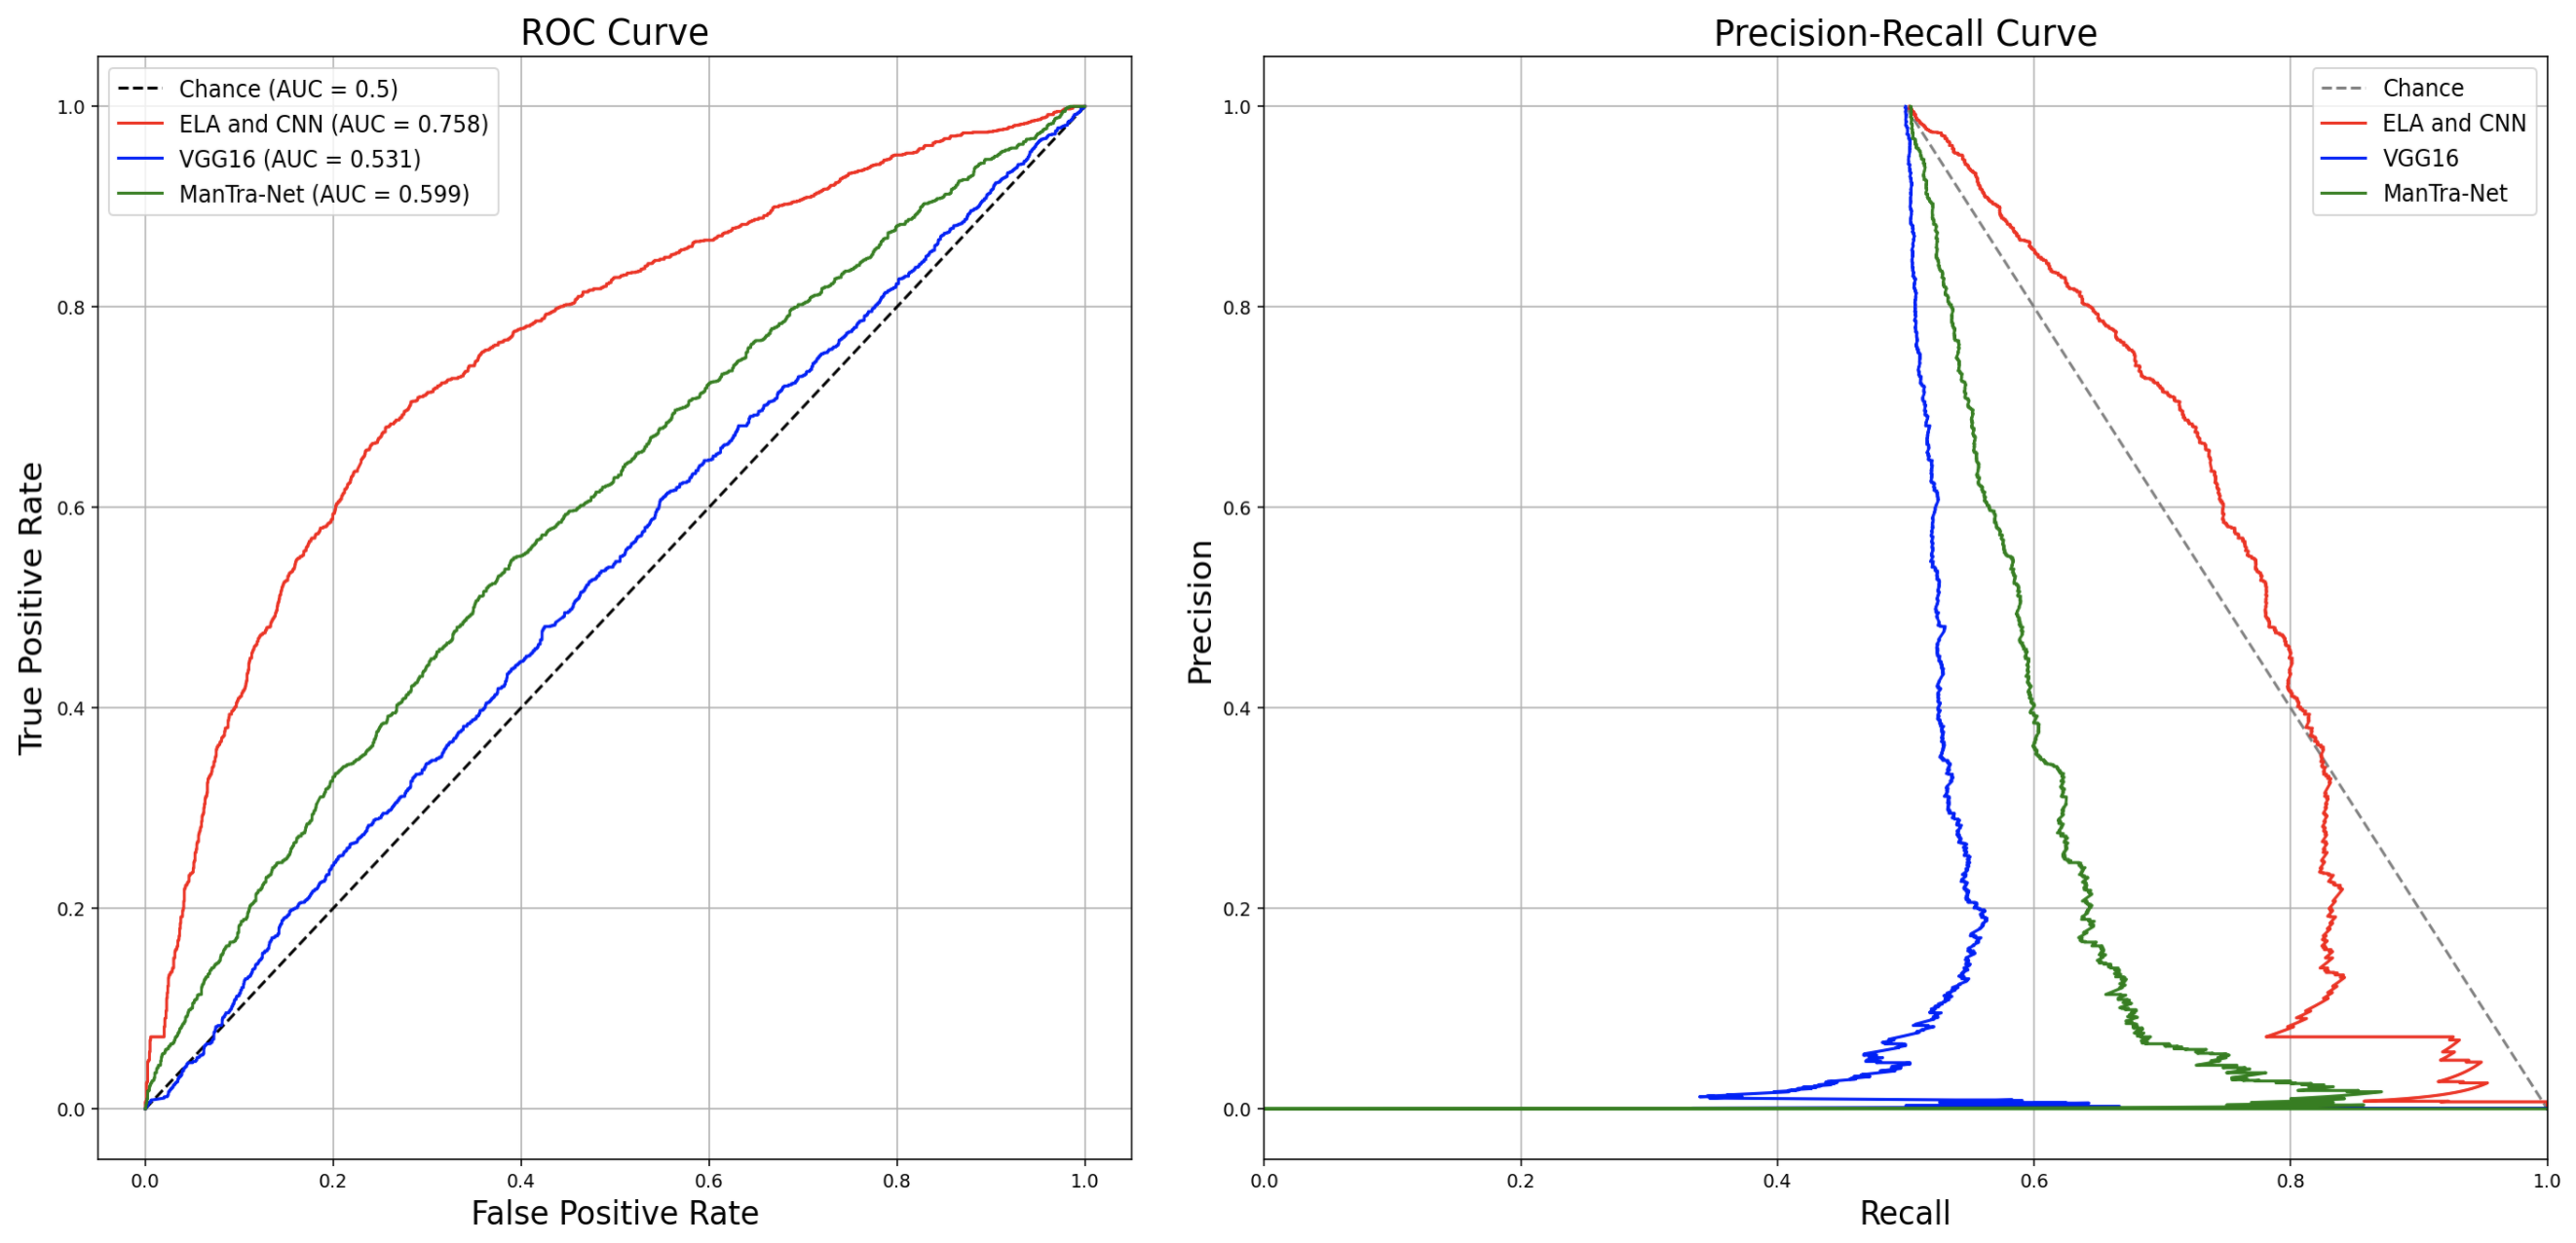
\includegraphics[scale=.31]{figures/figure_7.png}
    \caption{ROC-AUC curve (left) and precision-recall curve (right).}
    \label{fig:5}
\end{figure}

Since the ELA and CNN model performs the best in terms of both accuracy and AUC, we present the images where it does well and where it does not. Even though the ELA and CNN model performs best among other models that we tried, it still has a number of misclassifications. We can see in Figure 6 that this model can make true positive classifications when ELA fully captures the modified areas such as the halo beneath the swimmers and the toy on the dog’s head shown in Figure 6. And it can make true negative classifications when no modified areas are found by ELA or the highlighted areas are equally distributed across the image as shown in Figure 7.

\begin{figure}[!htb]
    \centering
        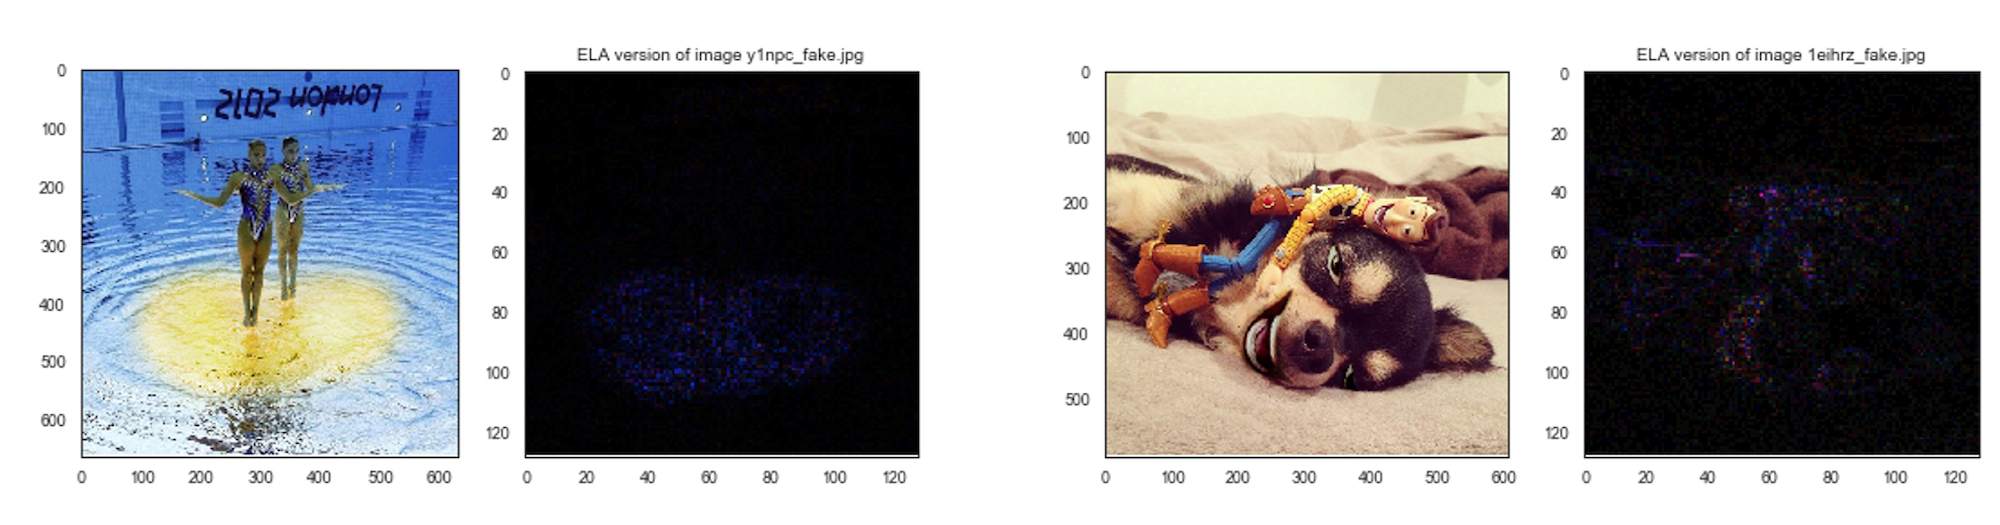
\includegraphics[scale=.42]{figures/figure_8.png}
    \caption{Examples of true positive classifications.}
    \label{fig:6}
\end{figure}

\begin{figure}[!htb]
    \centering
        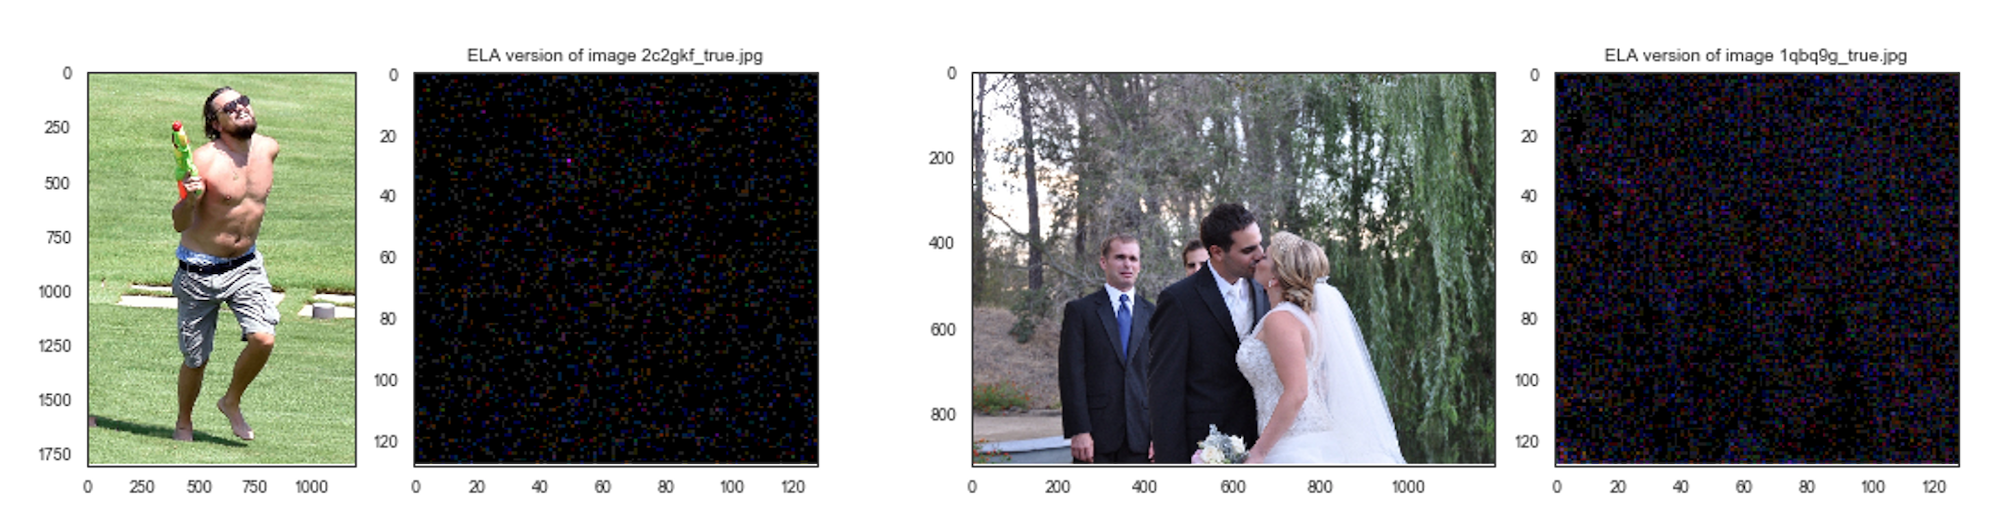
\includegraphics[scale=.42]{figures/figure_9.png}
    \caption{Examples of true negative classifications.}
    \label{fig:7}
\end{figure}

However, if there are densely scattered color contrast differences in the original image such as the strips on the leopard or the white text on the black background in Figure 8, ELA  assumes these areas are modified and highlight these areas, which later on causes CNN to classify them as fake images. On the other hand, if ELA fails to capture the modified area such as the elongated neck of the woman and the green bike in Figure 9, the ELA image is all dark, leading to false-negative classifications.

\begin{figure}[!htb]
    \centering
        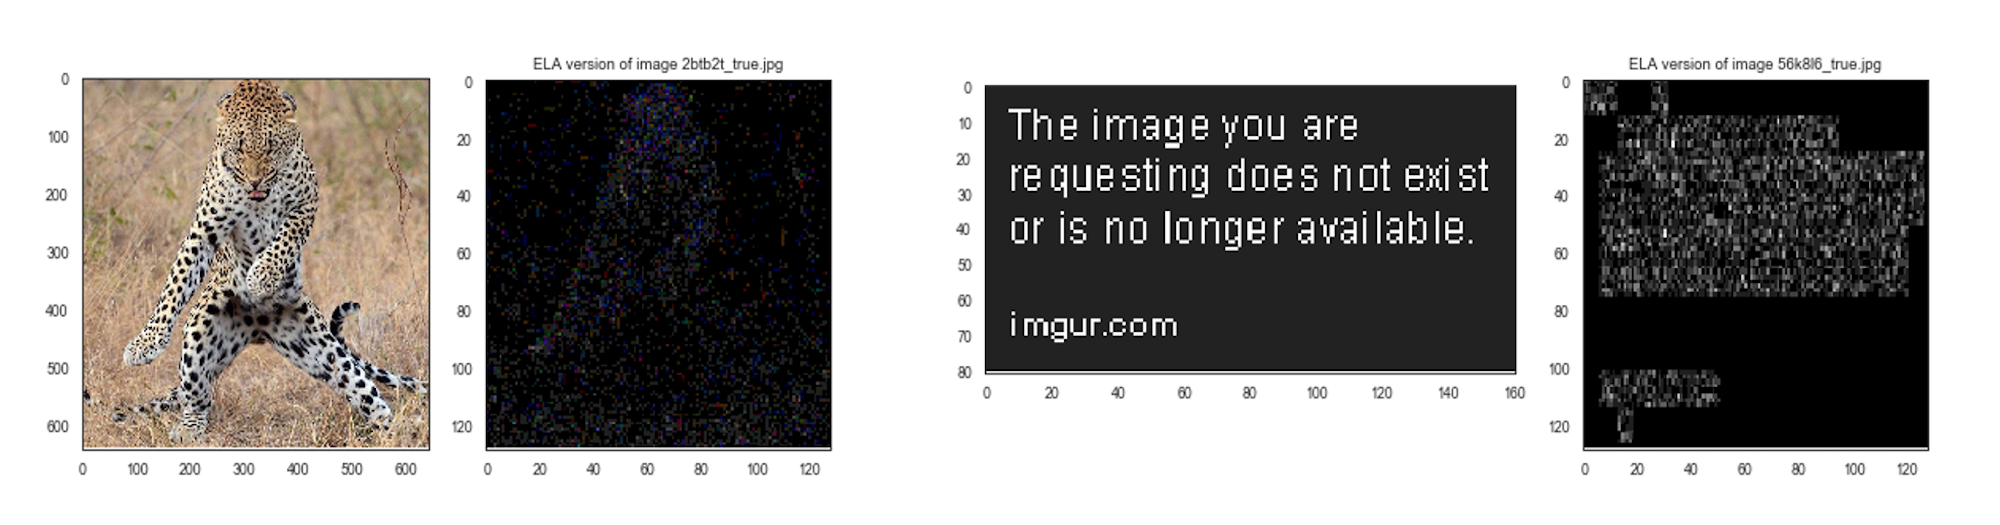
\includegraphics[scale=.42]{figures/figure_10.png}
    \caption{Examples of false positive classifications.}
    \label{fig:8}
\end{figure}

\begin{figure}[!htb]
    \centering
        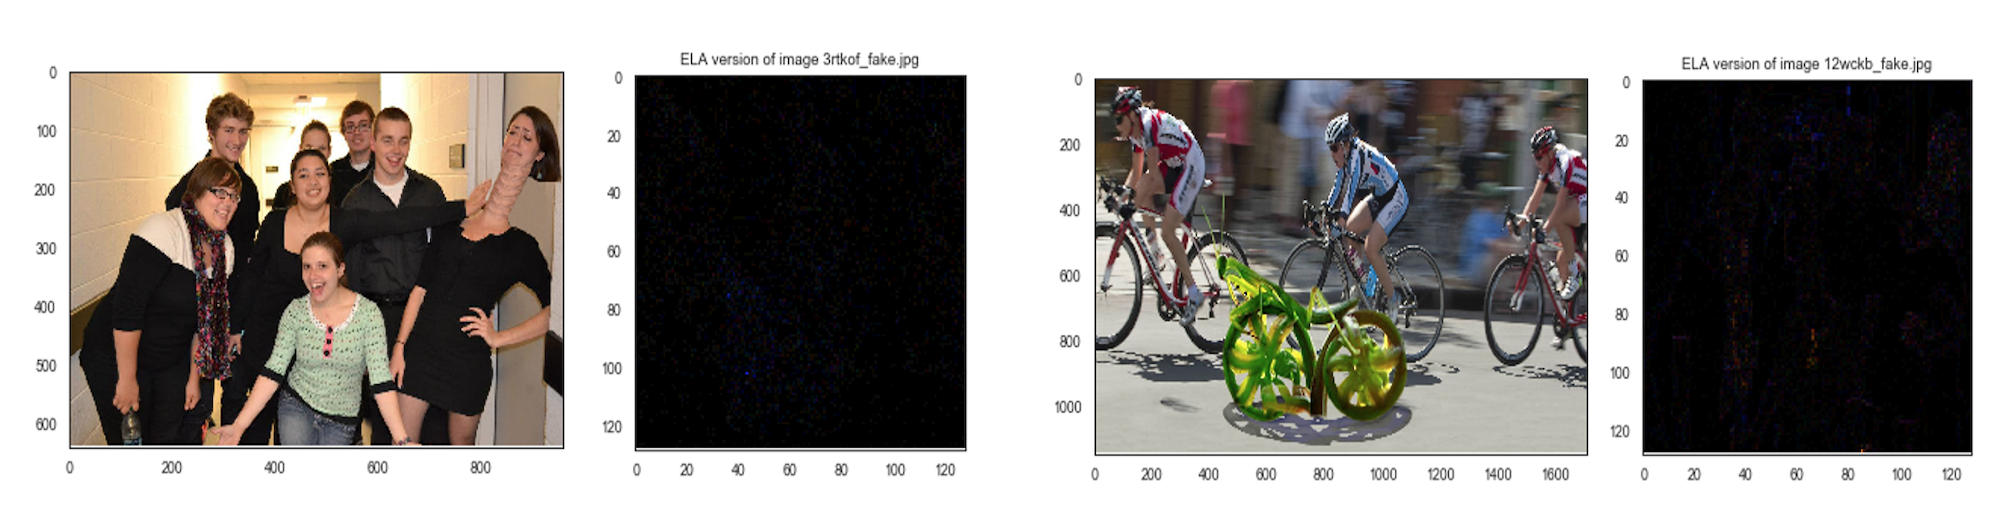
\includegraphics[scale=.42]{figures/figure_11.png}
    \caption{Examples of false negative classifications.}
    \label{fig:9}
\end{figure}

We also found that there are some images labeled as not manipulated that clearly is, as mentioned in the data section. Figure 10 is an example with men flying on brooms that is clearly manipulated but the dataset indicates it is not, which brings bias to our models, leading to lower accuracy for the model.

\begin{figure}[!htb]
    \centering
        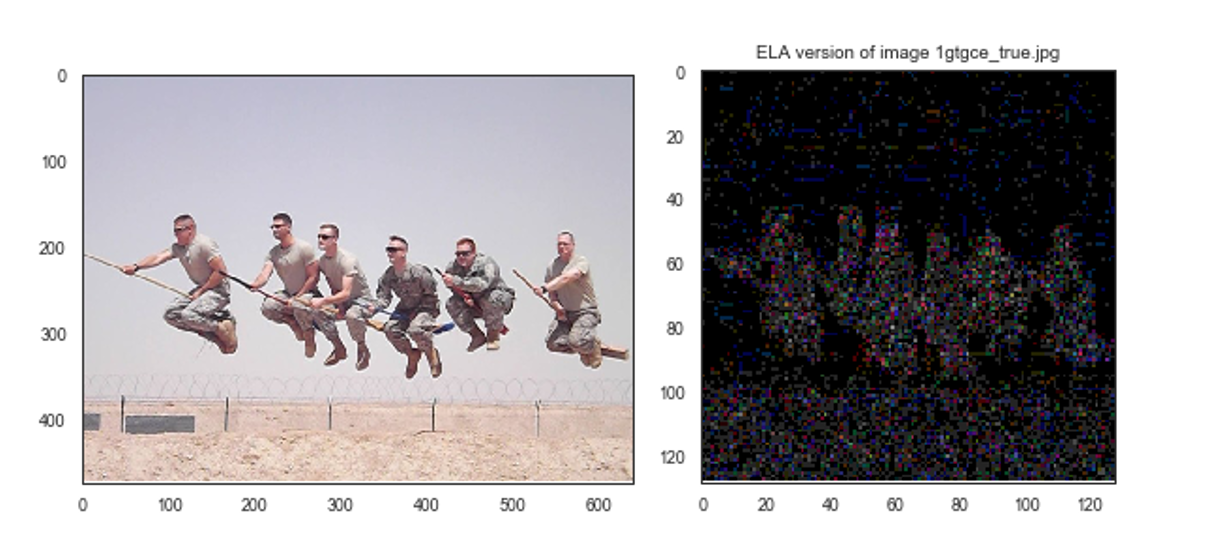
\includegraphics[scale=.75]{figures/figure_12.png}
    \caption{Examples of incorrectly labeled images.}
    \label{fig:10}
\end{figure}



% --------------------
\section{Conclusions}
% --------------------

After several iterations over diverse methods to accomplish the task proposed, the best method resulted to be the one integrating Error Level Analysis and Convolutional Neural Networks. The overall accuracy of the above model outperforms more complex transfer learning approaches but falls behind our custom human baseline. Nonetheless, it is important to mention that our human baseline for the PS-Battles dataset has potentially a high bias and a proofed wide confidence interval, since we did not calculate it using a rigorous statistical design as well as a well-formed sample of individuals. A more trustworthy metric to compare our model would the one presented by Nightingale et al. (2017), in which case our model improves human performance.

For further research, we would suggest using wavelet thresholding to remove the noisy components from the ELA-transformed images as well as trying to enhance ELA by using vertical and horizontal histograms, as noted in the literature review. Also, we would recommend implementing VGG16 with ELA-transformed images, as mentioned in the literature review, and see whether the results vary when we increase the resolution of the images significantly.  In addition, we could try other methods popular for forgery detection tasks, such as RGB-N and J-LSTM (Wu et al., 2019). Lastly, it would be interesting to see how the results would vary if we run our models on the original dataset without a perfect balance between original and fake images. We suppose that having several derivatives of the original image would add randomness to our dataset and could lead to better generalization of our models. However, due to the limited time and computational power, we could not implement these suggestions.


% %%%%%%%%%%%%%%%%%%%%%%%%%%%%%%%%%%%%%%%%%%%%%%%%%%%%%%%%%%
% %%%%%%%%%%%%%%%%%%%%%%%%%%%%%%%%%%%%%%%%%%%%%%%%%%%%%%%%%%
% REFERENCES SECTION
% %%%%%%%%%%%%%%%%%%%%%%%%%%%%%%%%%%%%%%%%%%%%%%%%%%%%%%%%%%
% %%%%%%%%%%%%%%%%%%%%%%%%%%%%%%%%%%%%%%%%%%%%%%%%%%%%%%%%%%
\medskip

\nocite{*}
\bibliographystyle{apacite}
\bibliography{references.bib}

\newpage

% --------------------
\section{Roles}
% --------------------

\begin{itemize}
    \item \textbf{Alena Kalodzitsa:}  I was responsible for producing the video for our team. This involved coming up with the idea for the video, scenes, writing some scripts, and video editing. Moreover, I have experimented with ELA to find optimal hyperparameters. I have also conducted an extensive literature review, suggesting trying ManTranNet on our dataset. Regarding the report, I wrote the background section, suggestions for further research (in conclusion), and wrote the description of the ELA method.  Lastly, I conducted a thorough review of our report, providing feedback, suggestions, and comments.
    \item \textbf{Amandeep Rathee:} I trained the VGGNet and ResNet models end-to-end with the help of the skeleton code created by Juan and the data created by Shota. I also conducted the human baseline study. In the report, I was responsible for writing part of the methods section (VGGNet and ResNet methods specifically along with creating the flowchart presented in the methods section). Further, I wrote part of the result section (aggregating the results from all models and human baseline study and presenting the accuracy, AUC and precision-recall for them).
    \item \textbf{Juan David Martinez:} I was the leader of the project and coordinated the different aspects of it. I took charge for the first version of the ELA + CNN strategy and coded the whole pipeline the team used throughout the project in Python. Also, I was responsible for Abstract, Introduction, Data and Conclusion sections of the report, as well as its formatting in \LaTeX.
    \item \textbf{Shota Takeshima:} I prepared the balanced dataset of true and forgery images. Also, I was in charge of the ManTra-Net + CNN model in terms of whole coding and tuning. For the presentation and report, I planned a rough constitution of our video and wrote about ManTraNet and CNN, and reviewed the whole report.
    \item \textbf{Xiao Lu:} I crafted the final model using ELA and CNN based on the pipeline Juan built, tuning the parameters for ELA and CNN to generate optimal results and add regularizations to prevent overfitting. In terms of the video presentation, I created the structured slides for video making and also wrote the video script. Regarding the report, I wrote section 4.1.
\end{itemize}


As a team, we used \href{https://github.com/arathee2/fake-or-not}{GitHub} for version control and Google Colab for creating deep learning models. The report formatting was done in \LaTeX \hspace{0.25mm} using \href{https://www.overleaf.com/read/pvdqzbpfdzzj
}{Overleaf}.

\newpage

\section{Appendix}

\subsection{Baseline model results}

As a baseline to compare our models, we asked five people\footnote{We thank Soumya Jha, Preeti Singh, Jashandeep Singh, Forum Shah, and Sadhna Singh for labeling the data that are used for the human baseline models. We used labelbox.com for collecting the labels.} to manually annotate 100 images from the test data. All of them labeled the same 100 images and did not know the true labels. The individual accuracies are 60\%, 69\%, 77\% 80\% and 89\%. The mean accuracy of these individual scores is presented in Table 1 and we call it the human aggregate model. We also created a human majority vote classifier where we compute the predicted label for an image by taking the mode of all five annotations. We call this method as the human ensemble model and present its accuracy in Table 1. Table 1 also contains the accuracies from all the deep learning models that we used. The human models do not have AUC scores because there are no probability scores associated with these two models.

\subsection{Transfer learning}

Transfer learning is a technique in deep learning where a neural network model that is trained for a particular problem is used on a different but related problem. This technique is particularly powerful when the number of training samples is not large enough to train your own neural network which is the case with the data in our problem. Popular pre-trained models that have proved to be robust in image classification tasks are VGGNet (Simonyan and Zisserman, 2015) and ResNet (He, Zhang, Ren and Sun, 2016) which we have used in trying to identify manipulated images. We also used ManTra-Net as it has proved effective in image forgery detection as mentioned in the literature review.

There are multiple ways to use a pre-trained model. We can either change weights and/or the architecture of the pre-trained model. One has the option to either update the weights to fine-tune it to suit a particular application, or to “freeze” the weights. The latter method is generally used when there is not enough training data to fine-tune the model. Similarly, one can either change the architecture or use it as it is. Generally, architecture is changed at the output side of a pre-trained network to make it suitable for the problem at hand.

The advantage of using transfer learning in our case is that pre-trained models do an exceptional job at extracting features from images that could be used to classify the images as fake or not. The earlier layers of the network extract preliminary features such as shapes and boundaries whereas the later layers are good at detecting complicated features such as the objects present in the image themselves.

\subsubsection{ManTra-Net and CNN}

ManTra-Net is a pre-trained CNN model. We take advantage of ManTra-Net as a feature extracting network, and then use a CNN that takes input from ManTra-Net to classify an input image as fake or not. Figure 11 shows the architecture of ManTra-Net. A ManTra-Net is a popular technique for forgery detection tasks because it can detect forged regions regardless of the types of manipulations (e.g., splicing, copy-move, removal, enhancement, and even unknown types). The input side of ManTra-Net is the image manipulation trace feature extractor, which is trained with a pristine base image and a combined dataset of each type of forgery.  It calculates forgery features for each pixel, and passes them to the local normality detection network. In the local normality detection network, a difference between a feature in a pixel and the average feature in all pixels and its standard deviation are calculated. Using z-scores based on these sample statistics, it evaluates whether a pixel is a part of a forgery region. ManTra-Net also can handle a forgery image that has multiple forgery regions in it by dividing the image into some windows and calculating the z-scores for each window.

\begin{figure}[!htb]
    \centering
        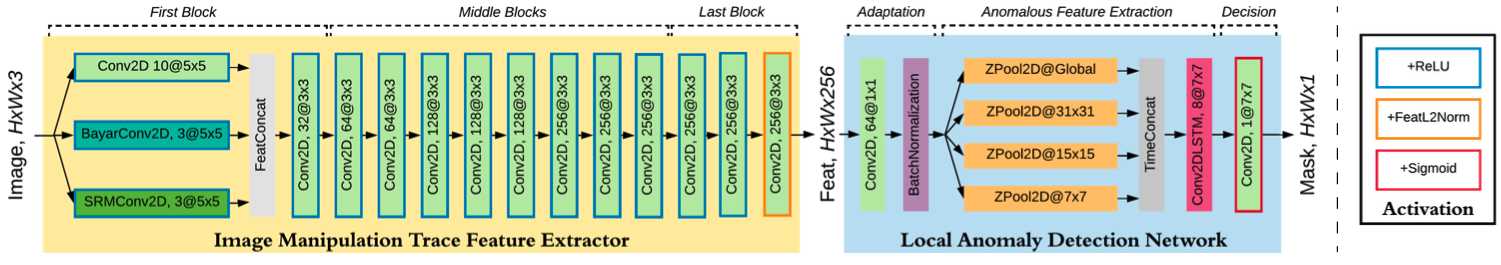
\includegraphics[scale=.28]{figures/figure_5.png}
    \caption{Architecture of ManTra-Net (reprinted from Conference on Computer Vision and Pattern Recognition (CVPR), Long Beach, CA, USA, 2019, pp. 9535-9544, Figure 2).}
    \label{fig:11}
\end{figure}

We also adopt a CNN classifier following ManTra-Net's feature extraction. The CNN we mentioned in 4.1 was too complex for these features and caused overfitting on the training dataset. Hence, after applying regularization and experimenting with simple architecture choices for the CNN, we adopted a network that is shown in Figure 12 (created using alexlenail.me software). The CNN takes input from ManTra-Net, applies a convolution and a pooling operation, followed by feeding the flattened output from pooling to a dense layer (50\% dropout ratio). The output of the dense layers is fed to the final layer that has two neurons corresponding to the probability of each class. We used RMSProp as an optimization strategy to get optimum weights for the network. For activating the outputs of each layer in the CNN, we used the ReLu function except in the output layer where a softmax function was used. Note that we only trained CNN and not ManTra-Net.

\begin{figure}[!htb]
    \centering
        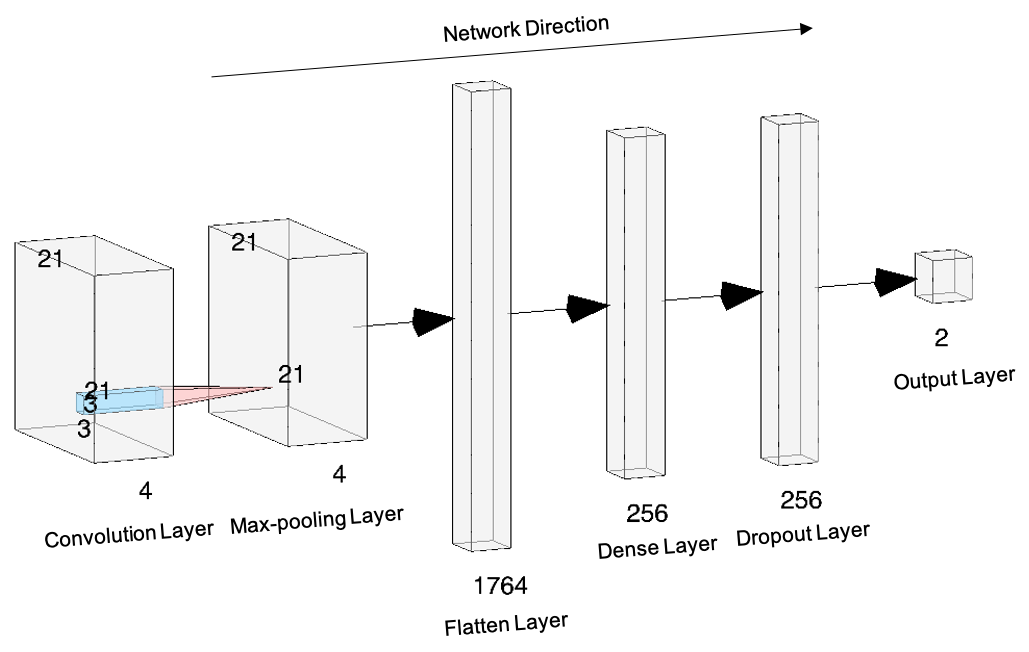
\includegraphics[scale=.65]{figures/figure_6.png}
    \caption{Complete Architecture of the CNN for features extracted by ManTra-Net.}
    \label{fig:12}
\end{figure}

\subsubsection{VGGNet and dense net}

We used a VGGNet-16 network (Simonyan and Zisserman, 2015) with pre-trained weights from the ImageNet competition. We replaced the fully connected layers present at the end of original VGGNet-16 with a dense network that has four fully connected layers because the VGGNet-16 was overfitting the training set. At the output layer of the VGGNet16, we used global max-pooling before moving to the fully connected dense network. A global max-pooling operation is a max pooling operation that reduces the size of feature space from (x, x, number of feature maps) to (1 x 1 x number of feature maps) by applying appropriate filter size. This reduction avoids the loss of spatial information that takes place when the output tensor from VGGNet-16 of size (x, x, number of feature maps) is fully connected to a dense layer.

The architecture of this entire model is shown in  Table 2. Each dense layer has L2 regularization with a penalty parameter of 0.001 (except for the last layer where we do not use L2 regularization as the model resulted in an inferior performance on unseen data). Each dense layer except the last one is followed by a ReLu activation and a batch normalization operation. Batch normalization results in faster convergence for the network parameters (Ioffe and Szegedy, 2015). The last layer uses a softmax activation with two neurons for the two classes. We used a batch size of 64 and trained the model for 125 epochs with binary cross entropy as the loss function. We saw no improvement in the training or validation accuracy after 125 epochs (until 150 epochs) which is why we chose 125 epochs.

While training the network, we tried updating the weights in just the dense network as well as the entire network. We found that when weights were “freezed” in the VGGNet-16, it was not able to even fit the training data well (since the accuracy on the validation set was the same as chance). For the dense network, we experimented with several fully connected layers and several choices of neurons in each layer before arriving at the optimal model. Increasing the number of layers did not have an impact on model performance a lot. When the number of neurons were higher than the ones presented in Table 2, the model started overfitting the training set. We also experimented with various regularization techniques such as dropout, L1 norm and L2 norm. In addition, we tried several activation functions but found that ReLu resulted in best performance. In all the networks, other than the one presented here,  resulted in an inferior performance on unseen data.


\begin{table}[!htb]
    \makegapedcells
    \centering
    \resizebox{\textwidth}{!}{%resizing the whole table
    \centering
    \begin{tabular}{|l|c|c|c|c|}
    \hline
        \textbf{Layer Operation} & \vtop{\hbox{\strut \textbf{Number of} }\hbox{\strut \textbf{Filters/Neurons}}}  & \textbf{Filter Size} & \textbf{Stride} & \vtop{\hbox{\strut \textbf{Resulting} }\hbox{\strut \textbf{Feature Size}}}  \\ \hline
        128 x 128 RGB input & - & - & - & 128 x 128 x 3 \\ \hline
        2 x convolutions & 64 & 3 x 3 & 2 & 128 x 128 x 64 \\ \hline
        max-pool & 64 & 2 x 2 & 0 & 64 x 64 x 64 \\ \hline
        2 x convolutions & 128 & 3 x 3 & 2 & 64 x 64 x 128 \\ \hline
        max-pool & 128 & 2 x 2 & 0 & 32 x 32 x 128 \\ \hline
        3 x convolutions & 256 & 3 x 3 & 2 & 32 x 32 x 256 \\ \hline
        max-pool & 256 & 2 x 2 & 0 & 16 x 16 x 256 \\ \hline
        3 x convolutions & 512 & 3 x 3 & 2 & 16 x 16 x 512 \\ \hline
        max-pool & 512 & 2 x 2 & 0 & 8 x 8 x 512 \\ \hline
        3 x convolutions & 512 & 3 x 3 & 2 & 8 x 8 x 512 \\ \hline
        max-pool & 512 & 2 x 2 & 0 & 4 x 4 x 512 \\ \hline
        max-pool & 512 & 512 x 512 & 0 & 1 x 1 x 512 \\ \hline
        fully-connected & 128 & - & - & - \\ \hline
        fully-connected & 128 & - & - & - \\ \hline
        fully-connected & 64 & - & - & - \\ \hline
        fully-connected (output) & 2 & - & - & - \\ \hline
\end{tabular}
    }
\caption{VGG16 and dense net architecture that is used to detect manipulated imagery.}
\end{table}

\subsubsection{ResNet and dense net}

In addition to methods presented above, we applied a deep residual network (He, Zhang, Ren, and Sun, 2016) in a similar manner as we used VGG16 network presented in section 8.2.2. After experimenting with several choices for a number of dense layers, activation function, regularization and optimization techniques, we found that ResNet did not fit the training set at all since it was doing as well as chance on the validation set. The model performance was similar to a model that predicts based on chance.

\end{document}
